\documentclass[12pt,letterpaper]{article}
\usepackage[utf8]{inputenc}
\usepackage{amsmath,amssymb,fullpage,graphicx}
\usepackage{subfigure}
\usepackage{amssymb}
\let\hat\widehat
\let\tilde\widetilde


\author{Nan Tang\\1662478}
	%% your name
\title{STAT 403 Spring 2018\\HW01}
	%% title of this document
\begin{document}
\maketitle
	%% make the title and author

\section*{Q1}

\subsection*{Q1-a}
	%% you can copy and paste your R code and result within the verbatim environment
%\begin{verbatim}
%\end{verbatim}

%%
%% Hint: using \includegraphics{FILENAME} to include a graph.
%% You need to place the figure to the same location as this template.
%%

\begin{align*}
Bias(\bar{X}) &= \mathbb{E}(\bar{X}) - \beta \\
&= \mathbb{E}(\frac{1}{n} \sum_{i=1}^{n}X_i) - \beta\\
&= \frac{1}{n} \sum_{i=1}^{n} \mathbb{E}(X_i) - \beta \\
&= \mathbb{E}(X_i) - \beta
\end{align*}

\noindent Note that $X$ follows an exponential distribution, the expected value for any sample from $X, X_i$ is equal to $\beta$.

\begin{align*}
Bias(\bar{X}) &= \beta - \beta = 0
\end{align*}

\noindent The sample average $\bar{X}$ is an unbiased estimator.

\begin{align*}
Var(\bar{X}) &= Var(\frac{1}{n} \sum_{i=1}^{n}X_i)) \\
&= \frac{1}{n^2} \sum_{i=1}^{n} Var(X_i) \\
\end{align*}

\noindent The variance of $X_i$ from exponential distribution is equal to $\beta^2$.

\begin{align*}
Var(\bar{X}) &= \frac{1}{n^2} \sum_{i=1}^{n} \beta^2 \\
&= \frac{\beta^2}{n}
\end{align*}

\noindent The variance of $\bar{X}$ is $\frac{\beta^2}{n}$.

\subsection*{Q1-b}

\begin{align*}
MSE(\bar{X}) &= Var(X) + Bias(X)^2
= \frac{\beta^2}{n} + 0 = \frac{\beta^2}{n}
\end{align*}

\noindent The mean square error of $\bar{X}$ is $\frac{\beta^2}{n}$.

\subsection*{Q1-c}

\noindent Note that $\lim_{n \to \infty} Var(\bar{X}) = \lim_{n \to \infty} \frac{\beta^2}{n} = 0$, since $\beta$ is fixed, and we have proved $\bar{X}$ is unbiased, $\bar{X}$ can be considered as a consistent estimator that converges to $\beta$ as sample size $n$ increases. 

\subsection*{Q1-d}

\begin{align*}
Bias(a \bar{X}) &= \mathbb{E}(a\bar{X}) - \beta \\
&= \mathbb{E}(\frac{a}{n} \sum_{i=1}^{n}X_i) - \beta\\
&= \frac{a}{n} \sum_{i=1}^{n} \mathbb{E}(X_i) - \beta \\
&= a \mathbb{E}(X_i) - \beta \\
&= (a - 1) \beta 
\end{align*}

\begin{align*}
Var(a \bar{X}) &= Var(\frac{a}{n} \sum_{i=1}^{n}X_i)) \\
&= \frac{a^2}{n^2} \sum_{i=1}^{n} Var(X_i) \\
&= \frac{a^2 \beta^2}{n}
\end{align*}

\begin{align*}
MSE(a \bar{X}) &=  Var(a \bar{X}) + Bias(a \bar{X})^2 \\
&= \frac{a^2 \beta^2}{n} + (a - 1)^2 \beta^2 \\
&= \beta^2 (\frac{a^2}{n} + (a-1)^2) 
\end{align*}

\noindent The mean square error for estimator $a \bar{X}$ is $\beta^2 (\frac{a^2}{n} + (a-1)^2)$.

\subsection*{Q1-e}

\begin{align*}
\frac{\partial MSE(a \bar{X))}}{{\partial a}} &= 2(a-1) \beta^2 + \frac{2a  \beta^2}{n}
\end{align*}

\begin{align*}
\frac{\partial^2 MSE(a \bar{X))}}{{\partial^2 a}} &= 2 \beta^2 + \frac{2 \beta^2}{n} > 0
\end{align*}

\noindent Since second derivative of $MSE(a \bar{X})$ is positive, we can get a minimum value of $MSE(a \bar{X})$ when $\frac{\partial MSE(a \bar{X))}}{{\partial a}} = 0$, then we obtain

\begin{align*}
2(a-1) \beta^2 + \frac{2a  \beta^2}{n} &= 0 \\
a &= \frac{n}{n+1}
\end{align*}

\noindent Substitute the value of $a$ into $MSE(a \bar{X})$

\begin{align*}
MSE(a \bar{X}) &= \beta^2 (\frac{(\frac{n}{n+1})^2}{n} + \frac{1}{(n+1)^2}) \\
&= \frac{\beta}{n+1} < \frac{\beta^2}{n} = MSE(\bar{X})
\end{align*}

\noindent The mean square error of $\bar{X}$ has its minimum value when $a = \frac{n}{n+1}$. Taking this value of $a$ minimizes $MSE(a \bar{X})$ so that the MSE of estimator $a \bar{X}$ is less than MSE of $\bar{X}$.

\newpage

\section*{Q2}

\begin{verbatim}
x_value <- seq(-10, 10, 0.05)
y_value <- exp(-sin(x_value)) * cos(pi * x_value)

plot(x_value, y_value, type = 'l', lwd = 2, col = 'goldenrod',
     xlab = 'x', ylab = 'y')
\end{verbatim}

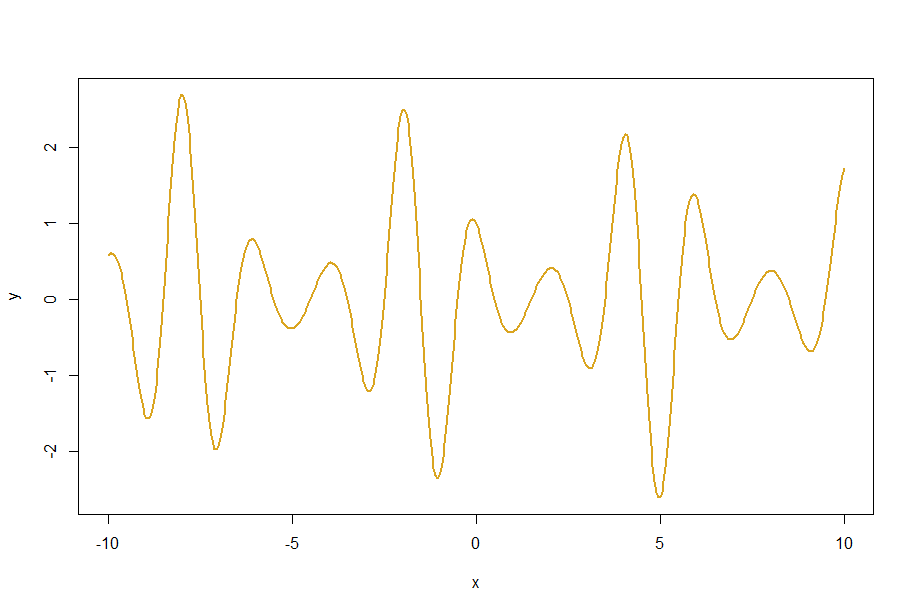
\includegraphics[width=150mm]{x-y_relation.png}

\newpage

\section*{Q3}

\begin{verbatim}
normal_dt <- rnorm(5000, 2, 2)
hist(normal_dt, breaks=50, main='Histogram of N(2, 2)', probability=TRUE, 
     col='powderblue')
x_nor_value <- seq(-5, 10, 0.01)
y_nor_value <- dnorm(x_nor_value, 2, 2)
lines(x_nor_value, y_nor_value, lwd=3, col='blueviolet')
\end{verbatim}

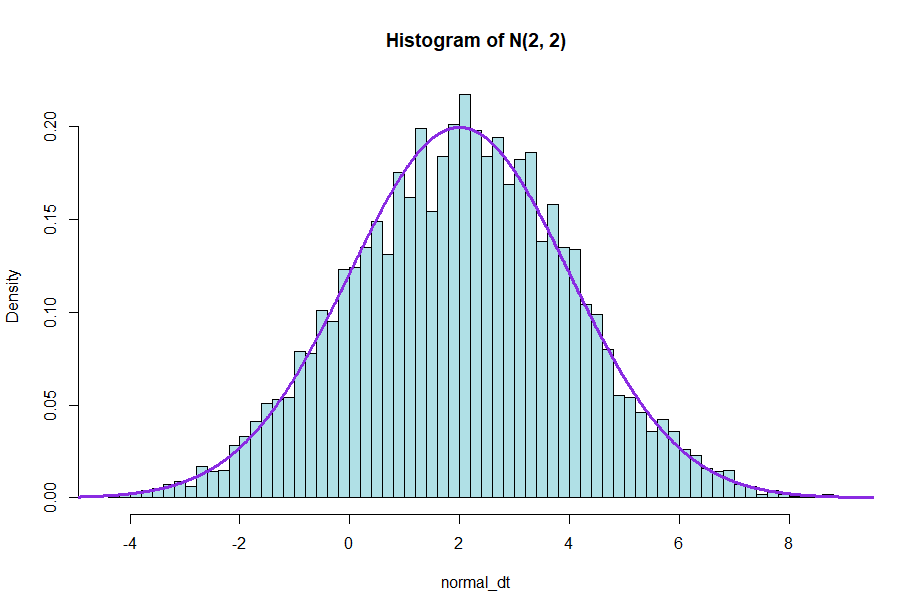
\includegraphics[width=150mm]{hist_norm.png}

\newpage

\section*{Q4}
\subsection*{Q4-a}

\begin{verbatim}
iterations <- 100000
unisample <- rep(NA, iterations)

for(i in 1:iterations) {
  uni_avg <- mean(runif(2, 2, 4))
  unisample[i] <- uni_avg
}

hist(unisample, breaks=50, main='Histogram of Sample Mean 
     of X1, X2 from Uniform(2, 4)', probability=TRUE, col='palegreen')
\end{verbatim}

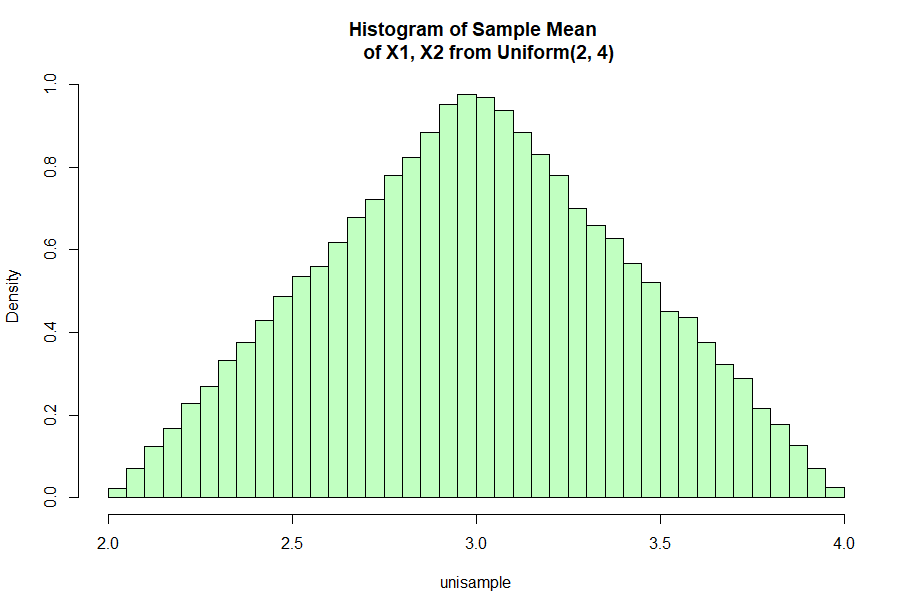
\includegraphics[width=150mm]{hist_unif.png}

\newpage

\subsection*{Q4-b}

\begin{verbatim}
hist(unisample, breaks=50, main='Histogram of Sample Mean 
     of X1, X2 from Uniform(2, 4)', probability=TRUE, col='darkseagreen1')
lines(c(2:3), c(0:1), lwd=3, col='deepskyblue')
lines(c(3:4), c(1:0), lwd=3, col='deepskyblue')
\end{verbatim}

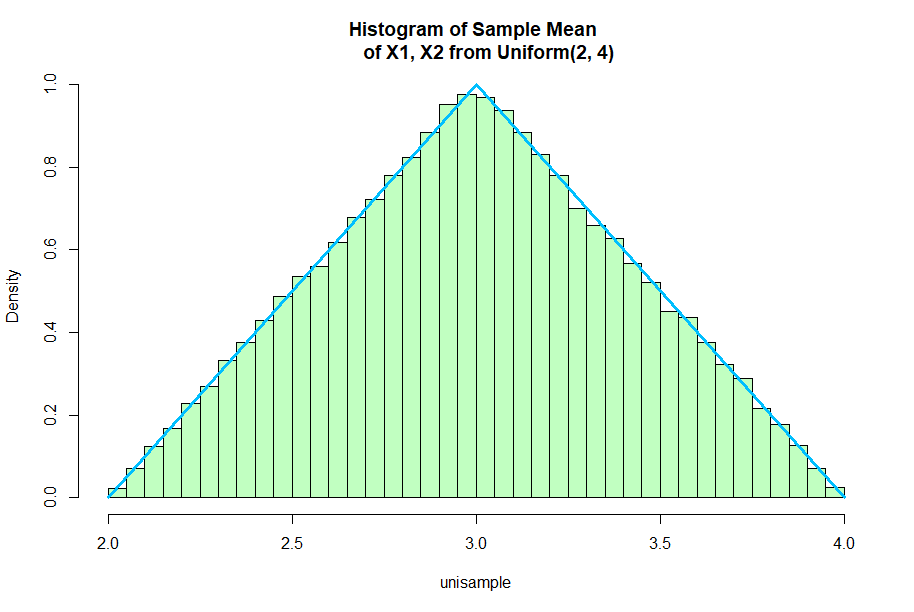
\includegraphics[width=150mm]{hist_with_dencurve.png}

%%% do not touch anything below
\end{document}
